\documentclass[12pt,oneside]{fithesis2}
\usepackage[english]{babel}
\usepackage[utf8]{inputenc}
\usepackage[T1]{fontenc}
\usepackage[shortlabels]{enumitem}
\usepackage[
scaled=0.86
]{berasans}
\usepackage[
scaled=1.03
]{inconsolata}
\usepackage[
plainpages = false,
pdfpagelabels
]{hyperref}
\usepackage{minted}
\usepackage[autostyle]{csquotes}
\usepackage[super]{nth}
\usepackage{blindtext}
\usepackage{graphicx}
\usepackage{float}
\setlist[enumerate]{font=\bfseries}
\usepackage{listings}
\usepackage{color}
\thesislang{en}
\thesistitle{Information systems integration and process optimization in a software company}
\thesissubtitle{Diploma Thesis}
\thesisstudent{Bc. Martin Jordán}
\thesiswoman{true}
\thesisfaculty{fi}
\thesisyear{Winter 2021}
\thesisadvisor{Ing. Leonard Walletzký, PhD.}
\graphicspath{{images/}}


\makeatletter
\usepackage{color}
\definecolor{lightgray}{rgb}{0.95, 0.95, 0.95}
\definecolor{darkgray}{rgb}{0.4, 0.4, 0.4}
%\definecolor{purple}{rgb}{0.65, 0.12, 0.82}
\definecolor{editorGray}{rgb}{0.95, 0.95, 0.95}
\definecolor{editorOcher}{rgb}{1, 0.5, 0} % #FF7F00 -> rgb(239, 169, 0)
\definecolor{editorGreen}{rgb}{0, 0.5, 0} % #007C00 -> rgb(0, 124, 0)
\definecolor{orange}{rgb}{1,0.45,0.13}		
\definecolor{olive}{rgb}{0.17,0.59,0.20}
\definecolor{brown}{rgb}{0.69,0.31,0.31}
\definecolor{purple}{rgb}{0.38,0.18,0.81}
\definecolor{lightblue}{rgb}{0.1,0.57,0.7}
\definecolor{lightred}{rgb}{1,0.4,0.5}
\usepackage{upquote}
\usepackage{listings}
\usepackage{biblatex}
\addbibresource{thebibliography.bib}
% CSS
\lstdefinelanguage{CSS}{
keywords={color,background-image:,margin,padding,font,weight,display,position,top,left,right,bottom,list,style,border,size,white,space,min,width, transition:, transform:, transition-property, transition-duration, transition-timing-function},	
sensitive=true,
morecomment=[l]{//},
morecomment=[s]{/*}{*/},
morestring=[b]',
morestring=[b]",
alsoletter={:},
alsodigit={-}
}

% JavaScript
\lstdefinelanguage{JavaScript}{
morekeywords={typeof, new, true, false, catch, function, return, null, catch, switch, var, if, in, while, do, else, case, break},
morecomment=[s]{/*}{*/},
morecomment=[l]//,
morestring=[b]",
morestring=[b]'
}

\lstdefinelanguage{HTML5}{
language=html,
sensitive=true,	
alsoletter={<>=-},	
morecomment=[s]{<!-}{-->},
tag=[s],
otherkeywords={
% General
>,
% Standard tags
<!DOCTYPE,
</html, <html, <head, <title, </title, <style, </style, <link, </head, <meta, />,
% body
</body, <body,
% Divs
</div, <div, </div>, 
% Paragraphs
</p, <p, </p>,
% scripts
</script, <script,
% More tags...
<canvas, /canvas>, <svg, <rect, <animateTransform, </rect>, </svg>, <video, <source, <iframe, </iframe>, </video>, <image, </image>, <header, </header, <article, </article
},
ndkeywords={
% General
=,
% HTML attributes
charset=, src=, id=, width=, height=, style=, type=, rel=, href=,
% SVG attributes
fill=, attributeName=, begin=, dur=, from=, to=, poster=, controls=, x=, y=, repeatCount=, xlink:href=,
% properties
margin:, padding:, background-image:, border:, top:, left:, position:, width:, height:, margin-top:, margin-bottom:, font-size:, line-height:,
% CSS3 properties
transform:, -moz-transform:, -webkit-transform:,
animation:, -webkit-animation:,
transition:,  transition-duration:, transition-property:, transition-timing-function:,
}
}

\lstdefinestyle{htmlcssjs} {%
% General design
%  backgroundcolor=\color{editorGray},
basicstyle={\footnotesize\ttfamily},   
frame=b,
% line-numbers
xleftmargin={0.75cm},
numbers=left,
stepnumber=1,
firstnumber=1,
numberfirstline=true,	
% Code design
identifierstyle=\color{black},
keywordstyle=\color{blue}\bfseries,
ndkeywordstyle=\color{editorGreen}\bfseries,
stringstyle=\color{editorOcher}\ttfamily,
commentstyle=\color{brown}\ttfamily,
% Code
language=HTML5,
alsolanguage=JavaScript,
alsodigit={.:;},	
tabsize=2,
showtabs=false,
showspaces=false,
showstringspaces=false,
extendedchars=true,
breaklines=true,
% German umlauts
literate=%
{Ö}{{\"O}}1
{Ä}{{\"A}}1
{Ü}{{\"U}}1
{ß}{{\ss}}1
{ü}{{\"u}}1
{ä}{{\"a}}1
{ö}{{\"o}}1
}
%
\lstdefinestyle{py} {%
language=python,
literate=%
*{0}{{{\color{lightred}0}}}1
{1}{{{\color{lightred}1}}}1
{2}{{{\color{lightred}2}}}1
{3}{{{\color{lightred}3}}}1
{4}{{{\color{lightred}4}}}1
{5}{{{\color{lightred}5}}}1
{6}{{{\color{lightred}6}}}1
{7}{{{\color{lightred}7}}}1
{8}{{{\color{lightred}8}}}1
{9}{{{\color{lightred}9}}}1,
basicstyle=\footnotesize\ttfamily, % Standardschrift
numbers=left,               % Ort der Zeilennummern
%numberstyle=\tiny,          % Stil der Zeilennummern
%stepnumber=2,               % Abstand zwischen den Zeilennummern
numbersep=5pt,              % Abstand der Nummern zum Text
tabsize=4,                  % Groesse von Tabs
extendedchars=true,         %
breaklines=true,            % Zeilen werden Umgebrochen
keywordstyle=\color{blue}\bfseries,
frame=b,
commentstyle=\color{brown}\itshape,
stringstyle=\color{editorOcher}\ttfamily, % Farbe der String
showspaces=false,           % Leerzeichen anzeigen ?
showtabs=false,             % Tabs anzeigen ?
xleftmargin=17pt,
framexleftmargin=17pt,
framexrightmargin=5pt,
framexbottommargin=4pt,
%backgroundcolor=\color{lightgray},
showstringspaces=false,      % Leerzeichen in Strings anzeigen ?
}%
%
\makeatother

\begin{document}
\FrontMatter
\ThesisTitlePage
\begin{ThesisDeclaration}
  \DeclarationText
  \AdvisorName
\end{ThesisDeclaration}
\begin{ThesisThanks}
  I would like to thank my supervisor Ing. Leonard Walletzký, PhD. for guidance, and for valuable professional and personal insights. Secondly, I would like to thank my wife, Jana Jordánová, who has been a tremendous mental support throughout all of my studies. This thesis would not be possible without the opportunity to work for Mautilus s.r.o. that has been given to me by Mr. Ivan Bradáč. A huge thank you also goes to all of my family members, who have been greatly supportive. I would also like to thank my father-in-law and mother-in-law for their words of encouragement.
\end{ThesisThanks}
The aim of this thesis is to integrate several systems in the selected company and to analyze and optimize processes in the financial department. Furthermore, it is to provide an evaluation of the added value of such implementation to the company, including the development of specific indicators to map this added value.
\begin{ThesisAbstract}
  This thesis deals with analysing, modelling and optimizing processes in the financial department and integrating several systems to improve a selected process. The subject is to analyze the processes, identify their inefficiencies and propose improvements. The stems from specific needs of a private company, therefore we examine the current state and suggest possible solutions. With the guidance of an indicator used to maximize the added value, we choose one of the processes to automate. Based on the collection of requirements we propose and implement a solution to that process. Finally, we evaluate the added value of our solution. An integral output of this thesis is an application that serves the purpose of automating the chosen process.
\end{ThesisAbstract}
\begin{ThesisKeyWords}Process modelling, Process optimization, Process automation, Finance, European Union funding programmes
\end{ThesisKeyWords}
\tableofcontents
\MainMatter
\chapter{Introduction}
In the recent years, video streaming services have taken the world by storm. This strong trend has been nothing but accelerated by the world pandemic. Therefore, it is no surprise that new, but also established companies are trying to capture their part of the market.
\par
When assessing whether a company is successful or not, we can look at many different metrics ranging from market share, through the number of monthly active users all the way to customer satisfaction. However, there is one general metric that stands above all - financial success. After all, the end goal of every company is to generate, continually increase and maximize profit over a sustained period of time.
\par
In the early stages, it can be difficult for a company to achieve positive financial results. To accelerate growth, companies are constantly searching for ways to acquire cheap capital, optimize their processes and reduce costs. One of the ways smaller companies can speed up their growth is to get acquired by a larger company. This inevitably creates additional complexities and side effects that, if not dealt with, may hinder the business in the long run.
\par
To drive innovation, European Union is offering funding programmes (sometimes also called calls) to companies in various areas of expertise. To be able to acquire these funds, firms must comply to a strict set of rules set by the European Commission.
\par
The main idea of this thesis is to analyze, optimize and automate certain tasks to remove unnecessary operational overhead from company employees. Because the complexity differs greatly between the analyzed processes, we will try to provide a common ground on which we can decide which process, if automated, will have the highest overall benefit to the company.
\newpage
\section{Thesis goals}
This thesis aims to analyze company processes in the financial department, their subsequent automations and possible systems integrations. One of the goals is to test the hypothesis of which one of the processes, if automated, is going to yield the highest overall results. To determine whether our hypothesis is correct we are going to create a common indicator. By extension, this indicator will point to the added value of this thesis. Finally, it is to implement a solution to the process identified by the indicator.
\section{Thesis structure}
The content of this paper is divided into seven chapters. The opening chapter serves as an introduction to better understand the domain within which this thesis operates. It describes the EU funding programmes and presents their motivation and goals in general. Furthermore, it introduces important concepts such as company size, job position relevance and annual work unit. The next chapter is dedicated to presenting the methodology of the thesis. The chapter after that analyzes the processes and presents the requirements for automating said processes. Following that, the optimized processes are presented together with some of the technologies used. Finally, the last chapter contains the implementation and deployment details.

\chapter{Theoretical framework}
In order for this thesis to not only seemingly have, but also show the added value, we have applied scientific methodologies to look for similarities and differences between our processes. In our closed environment, where we have a limited number of respondents, we mostly had to make do with opinionated data. Meaning that, to analyze the processes, we have collected the primary data through direct interviews with the employees that perform them.

With that in mind, we focused on qualitative research to be able to describe the processes and put them into models. This helped us identify the positive and negative outcome of dealing, or not dealing with the process automation. 

We applied the quantitative research method to gain insights into the time effort. While we certainly want to enrich the company with valuable insights 
While specifying the common indicator, we will try to be as objective as possible, letting the data guide us, rather than trying to find something in it.

In this chapter, two main methodologies that are commonly used to performing

\section{Conducted research}
Popsat obecně, co to je kvalitativní výzkum a pak konkrétně, jaké otázky jsme pokládali
Popsat obecně, co je kvantitativní výzkum a pak konkrétně jaká data jsme sbírali
\section{Business process management}
This will be a theoretical introduction into business processes and how the company is trying to apply this field of study.
"A business process consists of a set of activities that are performed in coordination in an organizational and technical environment. These activities jointly realize a business goal. Each business process is enacted by a single organization, but it may interact with business processes performed by other organizations."\cite{weske2007business}
\par
Hidden between the lines, there is much more to be found in this definition, than it would seem at the first sight. The one thing that a process also does, that is not mentioned in this definition and is certainly the case with all three of our processes, is that it transforms some input into some output. Let us now describe the processes and create their models with BPMN.\footnote{"Business Process Model and Notation is the standard for business processes diagrams. It is intended to be used directly by the stakeholders who design, manage and realize business processes, but at the same time be precise enough to allow BPMN diagrams to be translated into software process components. BPMN has an easy-to-use flowchart-like notation that is independent of any particular implementation environment."\cite{bpmn}} We will also define their inputs and outputs, which will greatly help us in creating our common indicator.

\chapter{Analysis and process modelling}
This chapter deals with analysing and modelling company processes. In the introductory section, we provide a general overview of the processes within the finance department and how they interact with different systems.

We identify the individual steps that make up these processes, what are their inputs and outputs and how they might affect other areas of the company.

//Based on this knowledge of these processes, we then identify areas of contact. This will naturally lead us into creating an indicator that will help us identify on which process we should be focusing and how, based on our goals and objectives aforementioned above in the section \ref{motivation}.

To accommodate for efficient planning, however, this data needs to be synchronized between the two systems.

\section{Systems overview}
In this section, we describe the systems the company uses to carry out daily operations and corresponding processes. Our focus here is on identifying the systems capabilities and recognizing the interactions between them. Currently, the company uses three separate systems for planning and tracking employee time. All of these systems have been in place since the two companies have merged.
\subsection*{BambooHR}
All-in-one HR software designed for small and medium businesses that makes it easy to collect, maintain, and analyze employee data, on-board new employees, manage compensations, and develop company culture.\cite{bambooHR} For us, it is important to know that this system enables employees to request time off and stores information about their contracts.
\subsection*{JIRA}
A comprehensive management suite for software development. It covers time planning, project roadmaps, issue tracking, release management and much more. The company currently uses JIRA server where the instance runs on their hardware. To track how employees actually spend their work time, the company uses Tempo Timesheets - an add-on for JIRA software.
\subsection*{Google Sheets}
A free cloud-based tool for creating and sharing cell-based tables. The company uses this for a yearly time availability outlook and quarterly planning. This is a solution the company started using during merging of two companies together. At that time, it seemed like a cheap and easy solution.
\subsection{Systems data flows}
In figure~\ref{fig:systems_dfd} we can see how the data flows from actors, through processes into respective systems. The idea here is to get a good grasp on the inputs and outputs for each of the processes and also to see the direction of the data flows with regards to the systems.

Any record of time being spent, be it time off or regular working hours is created by an employee.

For requesting time off, the input is one or more specific dates. After passing through the time off request process, this data is stored in BambooHR.

For submitting a time sheet, the time is accounted for on a per-task basis and enriched with complementary information. Specifically - to which project, issue and account the time belongs to. This data is then stored in JIRA.

To calculate the AWU, the finance controller has to take time sheets data from JIRA and contracts data from BambooHR.

In order for the assistant to synchronize the time off data they need to retrieve it from BambooHR and input it into Google documents planning sheet.

Finally, when planning, the managers consult the planning sheet for availability.

\begin{figure}[H]
    \centering
    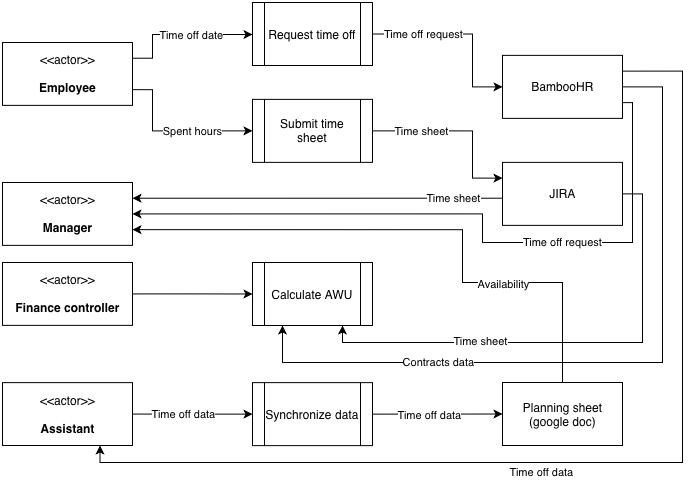
\includegraphics[width=\textwidth]{images/systems_dfd.jpg}
    \caption{Systems data flow diagram}
    \label{fig:systems_dfd}
\end{figure}

\section{Time reporting and planning}
In this section, we describe what happens when an employee wants to request time off and the effects it has on time reporting and regular planning meetings. First, we take a look at the procedure from broader perspective to gain a better understanding about how the processes influence each other. Then, we look at the sub-processes in more detail.

???Because the sub-processes are performed within different systems, they can be, and usually are, performed asynchronously.

The first key point of this process is that there are three different starting points. It can either start periodically every week - typically on Friday afternoon, when an employee wants to request some time off or when they have scheduled time off and want to cancel it. Depending on this, we get three different flows.

Using this approach, we want to demonstrate the fact that requesting time off can have impact on time sheet submission. For example - if an employee has a full week of vacation, it makes sense to submit their hours into both systems at once. Another example would be if an employee were in the middle of a vacation and suddenly decided to cancel the rest of it. Although not very common, these edge cases create unnecessary operational overhead. Furthermore, missing someone's vacation could potentially lead to inaccurate planning.

If this process is initiated by the regular weekly time reporting obligation, 

If an employee wants to request time off, they start by initiating the time off request process. The completion of this step leads to two things. Firstly, a notification is sent to an HR assistant triggering the synchronize data process.  This is essentially an asynchronous process, meaning that the ongoing process . This creates subsequent issues like the need for someone to be 

Secondly, the possibility to cancel a time off request arises. Choosing not to cancel the time off request leads to the time sheet submission process.

However, this diagram is not to be taken as a process that would be in accordance with our process definition and the BPMN standard. In this instance, we are just using the BPMN to explain the relationships more easily.


If the process starts 

If the process starts with an employee wanting time off, then it can have an impact on the output of the submit time sheet sub-process.

The figure shows 

\begin{figure}[H]
    \centering
    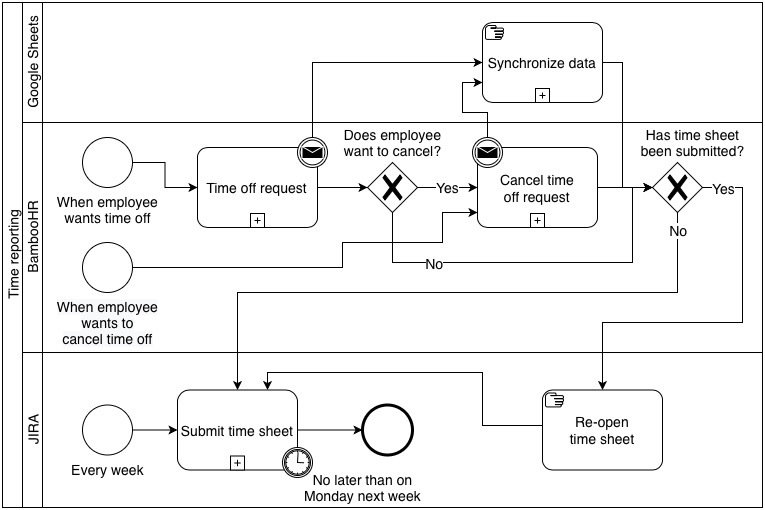
\includegraphics[width=\textwidth]{images/time_reporting.jpg}
    \caption{Time reporting}
    \label{fig:time_reporting}
\end{figure}

As we can see, there are many issues with the current state

\subsection*{Request time off}
In the diagram~\ref{fig:time_off_request} we can see the time off request process. An employee starts this process by submitting a time off request form in BambooHR. The input for this form is simply the amount of days and the type of time off the employee wants to request. After the request submission, the system automatically notifies corresponding manager via an email. The manager evaluates the request and decides whether to approve or deny it. If he chooses to reject the request, the process is terminated entirely and the system sends an email to the employee notifying them their request has been declined. If the request is approved, the system notifies the employee and an assistant about this.

\begin{figure}[H]
    \centering
    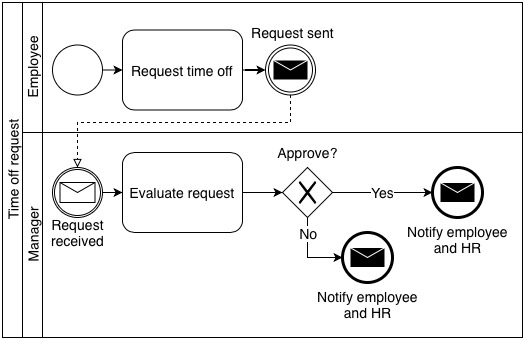
\includegraphics[width=\textwidth]{images/time_off_request.jpg}
    \caption{Request time off process}
    \label{fig:time_off_request}
\end{figure}

\subsection*{Cancel time off}
In some cases, it can happen that an employee wishes to cancel scheduled time off. Both \textit{approved} and \textit{pending for approval} time off requests can be canceled by the employee as long as the time of the leave is in the future. If not, the manager needs to delete such request by himself. This constraint is in place to protect time planning.

\begin{figure}[H]
    \centering
    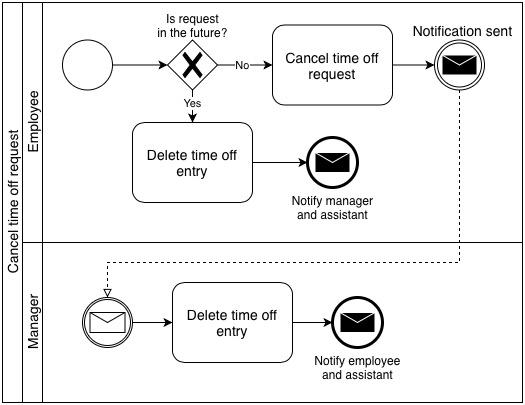
\includegraphics[width=\textwidth]{images/cancelling_time_off.jpg}
    \caption{Cancel time off}
    \label{fig:cancelling_time_off}
\end{figure}

\newpage
\subsection*{Submitting a time sheet}
In figure~\ref{fig:submit_timesheet} we can see the time sheet submission process - a standalone procedure that does not necessarily rely on being part of our time reporting diagram. The upper boundary for the input is defined by the employee's contract - sometimes also referred to as FTE. The main component is the time an employee spends working. Furthermore, vacation, special leave, public holidays, birthdays and other types of time off need to be included in this time sheet. It is essential for the output of this process to be accurate, reported in time and accounted against the correct accounts because the company uses the output for invoicing customers, employee payrolls and internal and external financial reporting purposes.

Throughout the day, employees input their hours into Tempo Timesheets. Then, usually at the end of the week, they submit this time sheet for approval but no later than on Monday the following week. The manager reviews this and either approves or requests a change. If he requests a change, a notification is sent to the employee, they make adjustments and re-submit the sheet. If the manager approves, the process finishes by again notifying the employee their time sheet has been approved.

\begin{figure}[H]
    \centering
    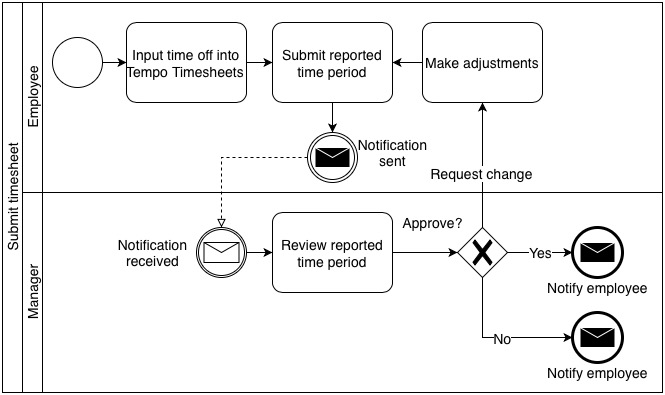
\includegraphics[width=\textwidth]{images/submit_timesheet.jpg}
    \caption{Timesheet submission process}
    \label{fig:submit_timesheet}
\end{figure}
\newpage
\subsection*{Synchronizing time off data}
In figure~\ref{fig:sync_vacation_to_gdoc}, we can see the data synchronization sub-process. This starts when an HR assistant receives an email with time off data. This can either be new time off or existing time off being canceled. First, they need to check whether there has been a contract change. If yes, they proceed to adjust the FTE. After this, they can synchronize the time off into the planning sheet.

\begin{figure}[H]
    \centering
    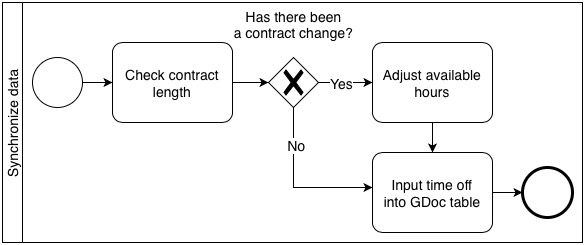
\includegraphics[width=\textwidth]{images/sync_vacation_to_gdoc.jpg}
    \caption{Time off synchronization process}
    \label{fig:sync_vacation_to_gdoc}
\end{figure}
After this is done, there is no notification sent to anyone and the only information of the time off being put in the planning sheet is in the sheet's history. Since the sheet contains planning data for all teams, the history gets cluttered and is practically unusable.
\newpage
---The problem becomes apparent when the need arises to transfer this data to a different system. After time off has been approved by the manager, a worker in the HR department receives an email notification. They then have to go and manually input this data into another system. Moreover, they have to update this data even when a request has been approved, but then subsequently removed due to some unexpected reason. In a sense, the assistant is acting as a synchronizing agent between the two systems.---


\section{Calculating annual work unit}
In the current state, in order to calculate the AWU, an employee has to manually export the data from accounting systems. Then, based on worker capacity, a decision has to be made whether or not to calculate the AWU internally, or outsource it to an external company. Regardless of which route we take, we always end up with a person having to manually copy data from one table to another in order to calculate the AWU. As such, we can say that both of these options are sub-optimal, as one carries workload overhead and the other creates increased costs. Both of which could be put to a better use, if we were to automate at least some parts of the process.

The following figure shows the process of calculating the AWU prior to creation of this thesis. It is clear that there are tasks which can be automated.
\begin{figure}[H]
    \centering
    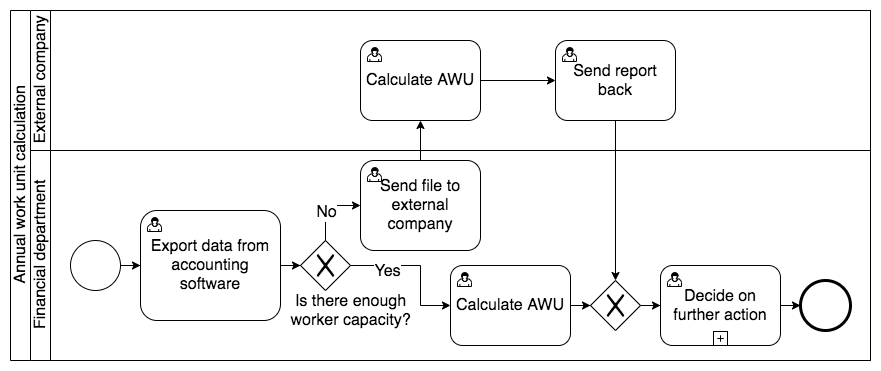
\includegraphics[width=\textwidth]{before_automation.png}
    \caption{Process before automation}
    \label{fig:before_automation}
\end{figure}

In this process, we are transforming an input - the history of our employee contracts into an output - annual work unit. Since we are doing it manually, we are also investing employee's time and subsequently, financial resources. 

Following what has been said in section \ref{motivation}, while keeping in mind this input -> output logic, we can already see that this process is going to be a hard contender when it comes to the return on investment.

\section{Summary}
We are looking for ways to simplify these processes in the company. The main pain point in the time reporting workflow is that the time off data does not synchronize between the systems automatically. This creates fragmentation and requires constant input from HR assistants and also an unnecessarily high amount of attention from employees and managers. Because the planning sheet is not integrated within the issue tracking system (JIRA) there is no simple way for the finance department to map the planned time to specific outputs. This also attributes to the lack of visibility on when new features will be delivered. Finally, it makes it hard to compare between planned time and actual time spent.

The second problem we see is with calculating the annual work unit. 

\chapter{Possible improvements}
With the increasing focus on providing software services Suggested solution should 

\section{Time reporting and planning}
To improve the time reporting and planning, we need to eliminate several impediments. First, we we need to make sure that time off is synchronized across all systems at all times. We are looking for a solution that makes one of the systems into a single source of truth from which the data propagates to other systems. Since the time off request starts in BambooHR, it makes sense to start exploring our possibilities there.

First, we take a look at some of the solutions that are currently available in the market and determine whether or not they are viable for our use case. The internet search for keywords: "Tempo Timesheets BambooHR integration" leads us to investigating following services:
\begin{itemize}
    \setlength\itemsep{0em}
    \item blendr.io 
    \item zapier
    \item BambooHR Integration for Jira
\end{itemize}

After reviewing these products, we came to the conclusion that the first two would not be viable options. Blendr \cite{blendr} Zapier does provide a trigger for new time off, however, there is no way of dealing with the request type. Moreover, there was no action that would correspond to our requirement of adding time to specific ticket.\cite{zapier}

\subsection*{Custom API integration}
Because all of the current systems provide API access, there is also the possibility to create a fully custom integration.


Vytvářet úplně custom řešení nedává smysl, protože problematika je rozsáhlejší, než se na první pohled zdálo. Navíc by ve výsledku bylo zahozeno, protože se plánuje přechod na JIRA Cloud. Jako možné řešení planningu v google sheetu se jeví tempo planner. Nicméně toto se neví, kdy přesně bude. Do té doby 


\subsection*{BambooHR Integration for Jira}
BambooHR Integration for Jira is a software solution developed by New Verve Consulting and distributed as an add-on through the Atlassian Marketplace. It is designed to synchronize data between BambooHR and Jira. The integration is available for Jira server only. Jira cloud is in the works with an estimated delivery of spring 2021. The cost of this integration is divided into tiers based on the number of users. Our company falls into the 250 users tier which comes at a fixed cost of \$1,760.00 with one year of maintenance included.

"When an employee requests time off in BambooHR, the app automatically records the request in Jira. This means that the teams can now consider employee time-off when scheduling work in Jira. It also means that scrum masters, project managers, and wider PMO are better informed and equipped to forecast accurate completion dates based on team capacity."\cite{bamboohr-jira-integration}

The setup and installation process is fairly straightforward and well documented. To connect the two systems together, an administrator needs to download and install the add-on into Jira instance. Then, they create an API key to authenticate with BambooHR and input BambooHR subdomain to connect.\\

\noindent The following options are available for import frequency:
\begin{enumerate}[itemsep=0mm]
    \item Daily at specified time
    \item Hourly
    \item Every 2, 4, 6, 12 hours
    \item Cron expression \footnote{Cron is a software utility used to schedule procedures to run periodically at a specific time.}
    \item No regular import
\end{enumerate}

Additionally, parameters like start date, year range and request types can also be set up. Another benefit of this solution is that it also integrates with Tempo Timesheets and can automatically create worklogs for approved time off requests.

\subsection*{Tempo Planner}
Tempo Planner is a planning tool that integrates into Jira in the same way as the previous product. Project managers, scrum masters and other employees can use it to plan work, see available capacity and reflect on planned vs actual time. The add-on is available for both Jira server and cloud. Since our company uses Jira server and has less than 250 employees, the cost for us is fixed at \$5,000.00 with one year of technical support.\\

\noindent Feature highlights:
\begin{enumerate}[itemsep=0mm]
    \item Plan and approve work or request time from other teams
    \item Access real-time overview of available resources
    \item Account for time off and holidays
    \item Compare planned vs actual to improve estimates and plans
    \item Report on resource capacity to see booked and available capacity of employees
\end{enumerate}


\section{Calculating the AWU}

\begin{figure}[ht]
    \centering
    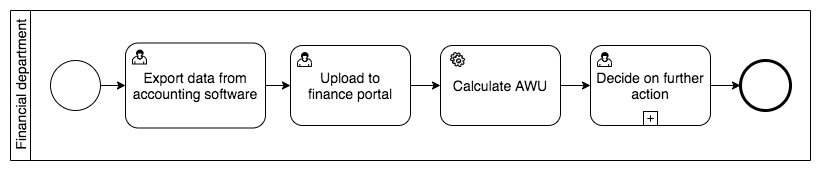
\includegraphics[width=\textwidth]{after_automation.png}
    \caption{Process after automation}
    \label{fig:after_automation}
\end{figure}

In BambooHR, we are looking for: 

In the documentation, we were looking for an endpoint that would provide us with 
The endpoint we are looking for is the "Time Off" endpoint.

\section{Summary}
Now that we have all of the possible solutions we can compare them and determine which one of them will provide us with the highest amount of added value for the least amount of resources spent. Any of these three 
Based on the comparisons we've we can now safely say that our initial hypothesis at the beginning of chapter \ref{hypothesis} was correct.

\chapter{Common indicator}
For us to be able to 
Let us define our common indicator as a combination of time effort, costs and potential savings.
Even though our processes overlap in some areas

Because we are dealing with multiple processes, we need to establish some common indicator to indicate how the changes affect our processes and what value they bring.

\section*{Time effort}
The first component of our indicator is time. 


In of these processes were being carried out manually by employees. This leads us to our first part of the indicator, time.
More specifically, two types of time:
An argument could be made against this that certain employees work faster than others and it might even sound right.
~\\\newline
We can see two concepts emerging from analyzing this process:
\begin{itemize}
    \setlength\itemsep{0em}
    \item How long does the task take to complete?
    \item How much time can we save if we don't do it?
\end{itemize}
 

\section*{Costs}
While the time effort can sometimes get unpredictable, we would generally not expect employee wage to fluctuate 

\noindent We have two types of costs:
\begin{itemize}[itemsep=0mm]
    \item Fixed - 
    \item Variable - employee salary
\end{itemize}
\section*{Potential gains}
In comparison to costs, gains are always potential, until they are realized. 


\section{Mapping indicator to processes}
\subsection*{Calculating the AWU}

\begin{center}
\begin{tabular}{ |c|c|c| } 
\hline
What & Before & After \\
\hline
Time spent & 1 & Janáček\\
Fixed costs & 2 & Smetana\\
Variable costs & 3 & Janáček\\
Cost per process execution & 2 & Janáček\\
\hline
\end{tabular}
\end{center}

\subsection*{Requesting time off}

For 214 employees there are 4 HR assistants whose responsibility is to take care . They are divided by locations so that each assistant has approximately equal number of employees. This makes 214 / 4 $\approx$ 53.

Since we cannot disclose exact salaries, we take 

\noindent We have two types of costs:
\begin{itemize}[itemsep=0mm]
    \item 2/4 assistants are from Czech with salary range between 29 - 57k CZK/month
    \item 1/4 is from the Netherlands with salary between 
    \item 1/4 is from the UK
\end{itemize}
\section*{Potential gains}
In comparison to costs, gains are always potential, until they are realized. 

\section{Evaluation}
To recapitulate, we have identified three different indicators. While they do provide some insight into which only when combined, create a meaningful and concise interpretation of 

\chapter{Systems integration}

\chapter{Process automation}
Now, we will describe the implementation. The chapter can be divided into four main sections:
\begin{enumerate}
    \setlength\itemsep{0em}
    \item Technologies
    \item Infrastructure and integrations
    \item Web application
    \item Data manipulations
\end{enumerate}

Because we are creating an application that is both front-facing and back-end oriented at the same time, it is important that we choose technologies that are mature and up to date.
When it comes to creating user interfaces, the ease of use and simplicity is very important both for the user and the developer. Because of this, I chose to use AWS Amplify in combination with GatsbyJS and React. Together, these three technologies make up the core of the front-end application. Amplify provides the infrastructure, GatsbyJS the routing and site generation and React ties it all together. Last but not least, we also want for the application to look at least somewhat decent and so we will also use component libraries to achieve a flat and pleasing look, stylized in company colors.
\section{Requirements}\label{hypothesis}
---(obsolete Intro)---
In the following paragraphs, the EU funding programmes domain is presented. The purpose of this is to familiarize the reader with the domain, so they can better understand the added value this thesis aims to provide. At this point we would like to state the hypothesis that we think that the winner will be the implementation of automating the task of calculating the Annual Work Unit.
\par
The conducted research is designed to examine the funding programmes, to provide an explanation as to why they are offered by the European Union (EU) in the first place and to identify their limitations and analyze their rules and conditions in order to be able to create a software solution that would help achieve the thesis goals. Also, the reasons why the company is taking part in the selected funding programmes are presented here.
\par
The analysis of the limitations and rules is achieved by collecting information from various different sources, including EU regulations, web sites and the Czech Civil Code as well as by interviewing the stakeholders. From a software engineering perspective, this process is called the Business Analysis.\footnote{"Business Analysis (BA) is the practice of enabling change in an organizational context, by defining needs and recommending solutions that deliver value to stakeholders."\cite{business-analysis}}
\par
In the first section, the EU funding programmes are introduced. Here, general motivation for the funding programmes is presented. After that, the terms medium-sized, small and micro enterprise together with the staff headcount and relevant and non-relevant job positions are defined. From these, the annual work unit (AWU) indicator is then derived. Furthermore, the specific conditions a company has to adhere to in order to be eligible. Finally, there is information as to why the company is applying for the specific programmes.
\newpage
The EU funding programmes are funding opportunities created by the European Commission to help micro, small and medium-sized enterprises (SMEs) gain access to cheap capital through grants, loans and guarantees. The companies can also bid for contracts to provide goods and services.
The specific project this thesis deals with is: "The company Mautilus, s.r.o. is implementing the project \textit{"New Apps Development in co. Mautilus"}, the goal of which is to develop multi-screen OTT (Over-the-top) applications designated for wide range of platforms that allow to watch video content." \cite{mau-eu-subsidy}
\subsection{(obsolete) Motivation for funding programmes}\label{motivation}
In this chapter, we will have a look at the motivations of both parties, the beneficiaries and benefactors. The former of which is our chosen company.
The Czech Civil Code considers: "A person who, on his own account and responsibility, independently carries out a gainful activity in the form of a trade or in a similar manner with the intention to do so consistently for profit is considered, with regard to this activity, to be an entrepreneur."\cite{entrepreneur-law}
\par
The quintessential part: "...carries out a gainful activity in the form of a trade or in a similar manner with the intention to do so consistently for profit..."\cite{entrepreneur-law} ties in well with the concept of financial leverage. \footnote{"Financial leverage, also known as leverage or trading on equity, refers to the use of debt to acquire additional assets."\cite{financial-leverage}} This concept is often used to accelerate growth.
\par
While it is entirely possible for a company to grow organically, it would be pointless to argue against obtaining cheap capital. Even more so, when the company does not have to accrue debt in order to acquire the resources. Therefore, funding programmes make perfect sense for SMEs, because they provide reasonable amounts of fairly accessible capital, while having no impact on the distribution of the company share.

This stands very true for our company as well, as it had received a substantial amount of funds. Not directly disclosed, yet publicly available.\cite{mautilus-funding}
\newline\newline
In the document: "Political Guidelines for the next European Commission" from \nth{15} July 2014, Jean-Claude Juncker, a Candidate for President of the European Comission stated the following: \blockquote{"Jobs, growth and investment will only return to Europe if we create the right regulatory environment and promote a climate of entrepreneurship and job creation. We must not stifle innovation and competitiveness with too prescriptive and too detailed regulations, notably when it comes to SMEs. They are the backbone of our economy, creating more than 85\% of new jobs in Europe and we have to free them from burdensome regulation."\cite{juncker-political-guidelines}}
In the year 2020, maybe more than ever before, we have seen that small businesses are a vital wheel in such a delicate and fragile machine that our economy undoubtedly is. It is not the purpose of this thesis to defend, nor argue against monetary policies and massive fiscal stimulus that we have seen in the past year. If anything, it is to demonstrate that European funds are being put to a good use. These lines portray the appetite European Union has for growth and innovation. Reading this, we can see a clear indication that growth, overall well being and abundance are the main motivators behind these funding calls.
\newline\newline
Also, in the same document, Mr. Juncker wrote: \blockquote{"Beyond that, I will leave other policy areas to the Member States where they are more legitimate and better equipped to give effective policy responses at national, regional or local level, in line with the principles of subsidiarity and proportionality. I want a European Union that is bigger and more ambitious on big things, and smaller and more modest on small things."\cite{juncker-political-guidelines}}
From the first part, we can see that Mr. Juncker has a genuine interest in enabling the Member States invest in their future. He then solidifies this by empowering them to take ownership of their local policies. He does all of this while maintaining a sober approach to such a delicate topic that is public resources.

To summarize, we can say that we see a genuine effort towards allocating public money in a fair and reasonable manner that is sustainable over the long term and helps small businesses grow into flourishing enterprises that solve real world problems. Without a doubt, this is a good enough motivation for such funding programmes to exist.

\subsection{Company size}
\noindent
According to the Commision regulation No.651/2014 \cite[page~70]{eu-commision-regulation} issued by the European Comission, the companies are divided into three categories according to the number of employees and annual turnover:
\begin{enumerate}
    \item Medium-sized enterprise
    \newline\newline
    Within the SME category, a medium-sized enterprise must have fewer than 250 employees and have an annual turnover not exceeding EUR 50 million, and/or an annual balance sheet not exceeding EUR 43 million.
    \item Small enterprise
    \newline\newline
    A small enterprise is defined as an enterprise which employs fewer than 50 persons and whose annual turnover and/or annual balance sheet total does not exceed EUR 10 million.
    \item Micro-enterprise
    \newline\newline
    A micro-enterprise is defined as an enterprise which employs fewer than 10 persons and whose annual turnover and/or annual balance sheet total does not exceed EUR 2 million.
\end{enumerate}
These figures apply to individual companies only. A small company might not qualify for SME status if it has significant additional resources because it is part of a larger group. \cite{eu-commision-regulation}
It is imperative for a company applying for a funding programme to fall into one of these three categories. If they don't, they are rejected. Our company falls into the small enterprise category.
\subsection{Job position relevance}
When applying for a programme, the relevance of a job position with respect to the project needs to be taken into account. Non-relevant employees are not accounted for in the AWU calculation. Nevertheless, it is useful to have this information.

It is also important to note that only employees working in the office that is listed in the application can be taken into account.\cite[page~30]{czech-rules}
\subsection*{Relevant (R)}
Employees, whose qualification and job are directly related to the project in question. (i.e. developers in our case)\cite[page~30]{czech-rules}
\subsection*{Non-relevant (N)}
All other employees fall into this category. (i.e. management, sales, accountants etc.)\cite[page~30]{czech-rules}
\subsection{Annual work unit (AWU)}
We have established that in order to be eligible for funding, a company has to have a certain amount of employees. Knowing only this would not suffice, as we need to take into account the time our employees have really worked. To enable this fine-grained distinction, European Union introduces the AWU.
\newline\newline
The European Comission defines the AWU as:
\blockquote{"...the number of persons who worked full- time within the enterprise in question or on its behalf during the entire reference year under consideration. The work of persons who have not worked the full year, the work of those who have worked part-time, regardless of duration, and the work of seasonal workers are counted as fractions of AWU."\cite[page~71]{eu-commision-regulation}}
\newpage
In practice, this means an employee's contract is represented on a scale from 0 to 1 where 0 means they are either currently not employed (i.e. an employee who resigned) or they have been on an unpaid leave. Conversely, 1 means they are working full time.

This means that the work of employees who have not worked the full year, the work of those who have worked part-time, regardless of the duration and the work of seasonal workers are counted as fractions of AWU.

~\\\newline
The staff consists of:
\begin{enumerate}[A)]
    \item employees;
    \item persons working for the enterprise being subordinated to it and deemed to be employees under national law; 26.6.2014 EN Official Journal of the European Union L 187/71;
    \item owner-managers;
\end{enumerate}
Apprentices or students engaged in vocational training with an apprenticeship or vocational training contract are not included as staff. The duration of maternity or parental leaves is not counted. \cite{eu-commision-regulation}
\section{Technologies}
The company is executing on it's mission to: "Innovate the way video-lovers discover, watch, and experience great content."\cite{24iMission} by using the latest and greatest technologies that are available on the market. To build it's infrastructure and services, the company uses Amazon Web Services (AWS). Because of this, it only made sense to also use AWS in this thesis.

The intent of this chapter is to provide a brief overview of the core technologies used in this thesis. More importantly, however, this list serves to demonstrate how these technologies have helped to achieve the thesis goals.

Amazon Web Services (AWS) is a branch of Amazon Inc. that provides a cloud computing platform and a variety of APIs to a broad range of customers, including companies and individuals alike. In it's entirety, AWS provides a set of abstract technical infrastructure and distributed computing building blocks and tools. This helps companies create solutions faster, more easily and with a higher degree of cost efficiency. \cite{what-is-aws} Thanks to the distributed nature and pay-as-you-go billing schemes, it is a fast and cheap way of delivering a highly scalable solution. \cite{aws-pricing}
\newline\newline
The main reason for using AWS in this thesis are the pre-prepared building blocks that were used to assemble a secure website while maintaining low costs. Also, it is the ability to consume desired API services in order to provide value to the company.
\subsection*{AWS Amplify}
AWS Amplify is a framework for creating full-stack applications in the cloud. It provides various different services such as Admin UI and AWS CLI, both of which can be used to initialize resources in the cloud. It also provides a library of React components that are directly connected to the other services like S3, API, or AWS Cognito.
\subsection*{GatsbyJS}
When used with React and GraphQL, GatsbyJS is a great tool for building web applications. Even though we are not using GraphQL we still chose to use GatsbyJS, because it provides a variety of different starters to help get a site up and running quickly.
\subsection*{AWS Lambda}
AWS Lambda is a serverless compute service that runs your code in response to events and automatically manages the underlying compute resources for you. You can use AWS Lambda to extend other AWS services with custom logic, or create your own back-end services that operate at AWS scale, performance, and security. AWS Lambda can automatically run code in response to multiple events, such as HTTP requests via Amazon API Gateway, modifications to objects in Amazon S3 buckets, table updates in Amazon DynamoDB, and state transitions in AWS Step Functions.
\subsection*{AWS S3}
AWS S3 is Amazon's cloud file storage. We are using it to store our files.
\subsection*{AWS Cognito}
AWS Cognito is an Authentication and Authorization service to manage user credentials and access to different cloud resources.
\subsection*{React}
React (also known as React.js or ReactJS) is an open-source, front end, JavaScript library for building application interfaces. It is maintained by Facebook and a community of individual developers and companies. React can be used as a base in the development of single-page or mobile applications. However, React is only concerned with rendering data to the DOM, and so creating React applications usually requires the use of additional libraries for state management and routing. Redux and React Router are respective examples of such libraries.
\par
I decided to use React to create the front end of the application mainly because I am using it every day as a part of my job, but also for it's ease of use and the ability to quickly develop a user interface.

In such a dynamic and ever changing environment, which information technology undoubtedly is, more and more companies are placing their emphasis on security, robustness and scalability of their IT systems. These are some of the attributes, which can be attained by migrating data to and consuming computational power from a cloud based solution thanks to it's distributed and modular architecture.

\section{Infrastructure}
In this section, we will briefly outline our infrastructure and environments.
\subsection*{Front-end environment}
The front-end of our application resides in the cloud that is managed by AWS Amplify. It automatically provisions an S3 bucket to store the source files. Then, a connection 
We have our GitHub repository connected to this environment. Every time a pull request is merged into the master branch, a deployment of 
\subsection*{Back-end environment}
The back-end consists of 4 services:
\begin{enumerate}
    \setlength\itemsep{0em}
    \item Authentication
    \item API
    \item Functions
    \item S3 Storage
\end{enumerate}
\section{Web application}
To automate the process of calculating the AWU, we are going to create a web application. To achieve this goal, we first need to be able to gather the data from the financial department. We will do this by providing them with a web application that fulfills all of the functional requirements described in the analysis.
To accommodate for user authentication, we leverage 

\subsection{Uploading a file}
Together with the file, we also need to collect some additional information about the data. Specifically, to which company and what year does the data correspond to.

\textit{\textbf{Dropdown}} This is a component from the popular library semantic-ui. It provides functionality to select a single, or multiple values, depending on the configuration. In this case, it gives us the ability to select one of the companies provided to it through options prop. After the user selects the desired value, an onChange event is fired, triggering the handleCompanyOptionChange method. In our application, we are also using it to select the desired year and as menu.

\begin{lstlisting}[style=htmlcssjs]
import { Dropdown } from 'semantic-ui-react'
<Dropdown
    selection
    options={companyOptions}
    defaultValue={company}
    onChange={this.handleCompanyOptionChange}
/>
\end{lstlisting}

\textit{\textbf{DropzoneDialog}} This component is a bit more complex. Implementing it from scratch would be overly complicated and completely unnecessary for our needs. It provides the means of selecting files from the computer file system either through file selection or drag and drop functionality. For our use-case, we chose to provide it with acceptedFile type of .xlsx and a filesLimit of 1, which, combined with selecting year and company creates a simple workflow.

\begin{lstlisting}[style=htmlcssjs]
import { DropzoneDialog } from 'material-ui-dropzone'
<DropzoneDialog
	open={open}
	onSave={this.handleSubmit}
	acceptedFiles={['.xlsx']}
	showPreviews={true}
	maxFileSize={5000000}
	filesLimit={1}
	onDrop={this.handleFileDropped}
	onDelete={this.handleFileDeleted}
	onClose={this.handleDialogClose}
/>
\end{lstlisting}

\textit{\large{parseAndUploadFile}} This method accepts an array of files of type File. It checks whether there are files in the array and if so, instantiates a new FileReader object that reads the file into memory. Then, on successfully loading executes the arrow function with the parameter e, which contains the resulting buffer. XLSX object from the eponymous library then uses its utility method sheetToCsv, which takes a worksheet. After this, fileName is retrieved from the component state and passed together with the file to the next method.

\begin{lstlisting}[style=htmlcssjs]
import XLSX from 'xlsx'
parseAndUploadFile = (files: File[]) => {
	if (files?.length) {
		const reader = new FileReader()
		reader.readAsArrayBuffer(files[0])
		reader.onload = e => {
			if (e.target) {
				const buffer = e.target.result
				const workbook = XLSX.read(buffer, { type: 'buffer' })
				const worksheet = workbook.Sheets[workbook.SheetNames[0]]
				const file = XLSX.utils.sheet_to_csv(worksheet)
				const { fileName } = this.state
				if (fileName) this.uploadFile(fileName, file)
			}
		}
	}
}
\end{lstlisting}

uploadFile This method takes a parameter fileName together with a file and invokes a put method on the Storage object, which has been imported from aws-amplify. The Storage object provides a means of accessing data objects stored in Amazon S3. Because it is linked directly to our back-end environment through configuration files, no other parameters are needed here, which makes it very easy on the developer.

After the file has been sent, the user is notified through an alert, indicating the upload was successful. Should the upload fail, an error is displayed. Because we are working on an internal tool, we can get away with less error handling as opposed if we were dealing with a commercial application. Nevertheless, it is a good practice to still show at least some information about what is going on with the application
\begin{lstlisting}[style=htmlcssjs]
import { Storage } from 'aws-amplify'
uploadFile = (fileName: string, file: string) => {
	Storage.put(fileName, file, {
		level: 'private',
		contentType: 'text/csv',
    })
	.then(result =>
		alert(
			`File: ${
				JSON.parse(JSON.stringify(result)).key
			} has been sucessfully uploaded`
		)
	)
	.catch(err =>
		alert(`Error: ${err} has occured, contact the administrator`)
	)
}
\end{lstlisting}

\subsection{Retrieving the AWU}
After the data has been uploaded, we also need to be able to retrieve the calculated results. We will now cover how this is handled on the client side.

fetchAnnualWorkUnit In this method, we first initialize the necessary parameters in order to be able to fetch the AWU. First, there is the apiName, which is a unique value used to identify the API we want to call. Then, the path is specified. There can be many paths on an API, but we only need just this one. Next, the authorization token is passed in the headers object. We need to do this so that we are able to use the back-end resources. Together with this, we also need to provide the user with some feedback while the data is being loaded. To do this, we have an isLoading boolean variable. This is used to display loading progress.

\begin{lstlisting}[style=htmlcssjs]
fetchAnnualWorkUnit = async () => {
	const apiName = 'api8df455ca'
	const path = `/awu`
	const params = {
		headers: {
			Authorization: `Bearer ${(await Auth.currentSession())
				.getIdToken()
				.getJwtToken()}`,
		},
		queryStringParameters: {
			company: this.state.company,
		},
	}
	this.setState({ isLoading: true })
	const response = await API.get(apiName, path, params)
	this.setState({ isLoading: false, data: response.data })
}
\end{lstlisting}


\subsection{Displaying the AWU}
Finally, we have to have some place for our computed data to be displayed. To do so, we again use a component from semantic-ui. This time, it is Table component.

Table This component takes on the following form and can be combined into many different styles of tables. For our purposes, we will use a traditional component with one headers row and a body, with the headers displayed at all times. The following code is just to show how the table can be used.

\begin{lstlisting}[style=htmlcssjs]
<Table>
	<Table.Header>
		<Table.Row>
			<Table.HeaderCell>Column name</Table.HeaderCell>
		</Table.Row>
	</Table.Header>
	<Table.Body>
		{data.map(item => (
			<Table.Row key={item.value}>
				<Table.Cell>{item.value}</Table.Cell>
			</Table.Row>
		))}
	</Table.Body>
</Table>
\end{lstlisting}

\subsection{Removing a file}
Dodělat!!!!!!

\section{Data manipulations}
To 
Even though the format transformation from .xlsx to .csv file has introduced some additional code complexity, the decision to do so has proved to be a good one, as the read speed of dataframe outpace the dataframe.readExcel almost eightfold. \cite{csv-read-speed}

\begin{lstlisting}

\end{lstlisting}

\subsection{Input data}
The employee data is gathered from an accounting system and exported in an excel file. The table below shows how the data is structured.

While there is some room for adjustments when it comes to the structure of the data we will be processing, we want avoid doing any manual interventions as much as possible. Because of this, we agreed with the finance department on a specific data format.

From our agreed upon data structure definition, 
\begin{center}
\begin{tabular}{ |c|c|c|c|c|c|c|c| } 
\hline
ID & Surname & Name & Type & January & February & ... & December \\
\hline
1 & Smetana & Bedřich & R & 1 & 1 & ... & 1\\ 
2 & Janáček & Leoš & N & 0.5 & 1 & ... & 1\\ 
3 & Karel & Borovský & R & 0.5 & 1 & ... & 1\\ 
\hline
\end{tabular}
\end{center}

readPrivateFile To retrieve the files with this data, we have the following portion of python code. It fetches the file from an S3 bucket based on the company and the year that is provided to it.

\begin{minted}{python}
def read_private_csv(company, year):
    key = '{}/{}/{}.csv'.format(my_prefix, company, year)
    response = s3.get_object(Bucket=my_bucket, Key=key)
    df = pandas.read_csv(response['Body'])
    df.columns = df.columns = df.columns[:4].to_list() + months_en
    rename_cols(4, df, '/{}'.format(year))
    df = df[df['Osobní číslo'].notna()].fillna(0)
    return df
\end{minted}

\subsection{Data manipulations}
The following snippet is the most important part of the python code. It takes a dataframe and an array of months in the format of: "MONTH/YEAR" and iterates over all "monthyears" to compute the average annual work unit for each month. After this, there are some more transformations to manipulate the data into output format.

\begin{minted}{python}
def get_averages(df, all_months):
    relevant = []
    non_relevant = []
    n_valid = []
    r_averages = []
    n_averages = []
    number_of_months = 12
    for index, item in enumerate(all_months):
        relevant.append(
            float(get_df_by_contract_type(df, 'R')[item].sum())
        )
        non_relevant.append(
            str(get_df_by_contract_type(df, 'N')[item].sum())
        )
        if index < number_of_months:
            r_averages.append('-')
            n_averages.append('-')
        else:
            r_averages.append(
                float(average(
                    relevant[index-number_of_months:index]
                ))
            )
        if int(float(non_relevant[index])) < 2:
            n_valid.append(False)
        else:
            n_valid.append(True)
    return [all_months, relevant, non_relevant, n_valid, r_averages]
\end{minted}

\subsection{Output data}
The following is the structure in which the data is presented to the user. The number this has all been done for is in the "1 year R average" column.
\begin{center}
\begin{tabular}{ |c|c|c|c|c| } 
\hline
Period & R & N & N > 2 & 1 year R average \\
\hline
january/2017 & 14 & 1.75 & false & - \\
\dots & \dots & \dots & \dots & \dots \\
december/2017 & 15 & 2.75 & true & - \\
january/2018 & 14 & 1.75 & false & 14.15833 \\
\dots & \dots & \dots & \dots & \dots \\
\hline
\end{tabular}
\end{center}
\section{Future development}
As a part of this thesis, we have implemented automation for calculating the AWU - one of the three processes we analyzed. We can already say that there is a bright future for this project, as the stakeholders like the simplicity and are interested in expanding the functionalities. Should that be the case, we would probably need to make adjustments to the way the data is being stored and handled, as that was good enough for the time being, but could quickly grow.

When it comes to the integration of Jira Temposheets and BambooHR, there is some attentiveness for this to be implemented, but because the current solution to the problem doesn't create any necessary costs, there is little to interest in doing so early.

Finally, no decision has yet been made on the matter of the tax forms process, as the department has recently undergone major restructuring. From a financial perspective, the tax forms process makes more sense to take precedence, as accounting department positions are generally better paying than assistants. Moreover, there is clearly a high amount of workload that could be better spent elsewhere, should this integration materialize.
\chapter{Conclusion}
The goal of this thesis was to analyze, model and identify possible optimizations and automations of three processes within the company. To better understand the value hidden underneath the possible process automations, we have developed a common indicator. This indicator has proved to be successful at determining which process to automate.

This thesis is a part of my so far, 2 year long employment contract with the company Mautilus s.r.o. Because I started on a part-time contract as a student, there has always been the the option, or rather almost an obligation, to create my thesis for the at the company. After all, it was one of the topics we discussed at the job interview. Since the beginning, I've been interested in helping the company be more efficient and I hope this thesis is a testament to that effort.
\printbibliography
\listoffigures
\end{document}


